\documentclass[12pt]{article}
\usepackage[T1]{fontenc}
\usepackage[margin=1in]{geometry}
\usepackage{booktabs}
\usepackage[table]{xcolor}
\usepackage{graphicx}
\usepackage{caption}
\usepackage{subcaption}
\usepackage{amsmath}
\usepackage{amssymb}
\usepackage{makecell}
\usepackage{setspace}
\usepackage{adjustbox}
% Reduce overfull-hbox warnings from long texttt identifiers and URLs.
\emergencystretch=3em
\hyphenpenalty=200
\tolerance=600
\sloppy
\usepackage[round,authoryear]{natbib}
\usepackage{hyperref}
\hypersetup{
    colorlinks=true,
    linkcolor=blue,
    citecolor=blue,
    urlcolor=blue
}
\doublespacing

\title{The Post-ChatGPT Contraction Reaches the Crowd-Validated Margin:\\
A Within-Tag Triple Difference and a Value-Calibrated
Early-Warning System for Stack Overflow}
\author{Henry Laverde-Rojas \quad Carlos Laverde-Rodriguez \\
Programa de Econom\'ia, Universidad Militar Nueva Granada, Campus, Colombia}
\date{\today}

\begin{document}
\maketitle

\begin{abstract}
\noindent
Generative AI has contracted public Q\&A activity on Stack
Overflow \citep{burtch2024chatgpt,delriochanona2024large,xue2026chatgpt};
a benign reading holds that it prunes only the low-value posts
a platform would not have retained as durable artefacts. Using
a primary 2020--2024 panel of 8.4 million Stack Overflow
questions across 100 top pre-treatment tags and 261 weeks, with
a full 100-tag 2025 validation extension, we estimate a
within-tag triple difference at the (tag $\times$ week
$\times$ question-type) cell. A pre-specified shape test
rejects the \emph{strict} benign reading: displacement is
negative across the crowd-validated range
($\hat\beta=-0.167$, $p<10^{-4}$), roughly constant over
the low-to-mid net-score bins and fading only at the rare
elite tail, so the channel reaches the crowd-validated margin
rather than being confined to score-zero posts. The volume
baseline is $-0.108$ ($p=0.021$) under a historical
answerability proxy and $-0.119$ ($p<0.001$) under a co-primary
embedding score that uses no historical features. We turn the
result into a \emph{value-calibrated early-warning system} for
budget-constrained allocation of intervention effort: out of
sample, the activity-decline metric a platform already tracks
detects where realised 2025 high-value erosion is largest
(AUC $0.98$; a value-weighted ranking reaches $0.57$), and the
value-margin estimates supply the \emph{calibration} that
converts an activity alert into the high-value posts at
risk---allocating effort by raw activity leaves up to $5\%$ of
the protectable high-value flow unprotected, while a persistent
composition flag ($\rho=0.90$ into 2025) classifies which
declines are value-disproportionate. Exact parallel trends are
rejected, so the estimate is a conditional post-ChatGPT
association aligned with the LLM-substitutability mechanism;
its credibility rests on a convergence of diagnostics---placebo
sign-reversal, pre-trend matching, a 32-cell specification
curve, a donut difference-in-differences, and a HonestDiD
breakdown at $\bar M=0.75$---and the full 100-tag 2025 extension
strengthens the triple difference to $-0.172$ ($p=0.002$),
deepening monotonically to $-0.68$ with no reversion. All
evidence for the main claims is reported in the article; a
public replication package provides the code, data-construction
scripts, audit logs, and extended robustness outputs.
\end{abstract}

\noindent\textbf{Keywords:} generative artificial
intelligence; large language models; online knowledge
communities; question-and-answer platforms; user-generated
content; digital public goods; innovation inputs;
crowd validation; triple difference;
pre-trend sensitivity.

\noindent\textbf{JEL codes:} O33, O36, L17, J24, C23, D85.

\section{Introduction}\label{sec:intro}
\label{sec:intro_body}

Public question-and-answer platforms such as Stack Overflow are
part of the digital infrastructure of distributed
problem-solving: they convert individual software problems into
searchable, accepted, moderator-retained posts that future
contributors, users, and---increasingly---large language models
consult when facing analogous problems
\citep{wasko2005faraj,goes2014popularity,nagle2018learning}.
Generative AI reconfigures this infrastructure: since November
2022 a wide class of programming questions can be routed to a
private conversational LLM at near-zero marginal search cost
\citep{eloundou2024gpts,acemoglu2024simple}, and that private
channel produces no public artefact unless the user voluntarily
reposts the resolved problem. The substitution between the public
and private channels---and its consequences for a platform whose
replenishment depends on the contribution incentives the
substitute now competes against
\citep{kankanhalli2005contributing,butler2001membership,benkler2002coase}---is
the question this paper studies.

Recent work establishes that aggregate replenishment has slowed.
\citet{delriochanona2024large} report a $\sim$15\% mean decline
rising to $\sim$25\%; \citet{burtch2024chatgpt} document
analogous declines across Q\&A platforms; and
\citet{quinngutt2024heterogeneous} report that the effect of
generative AI on knowledge seeking is heterogeneous rather than
uniform, motivating a move beyond a single average effect to the
within-community margin. \citet{xue2026chatgpt}, in \emph{ISR},
use a cross-platform design and document both a volume reduction
and an \emph{improvement} in the average quality of surviving
questions---a combination naturally read as \emph{benign
pruning}, under which LLMs absorb the easier, lower-value
questions. A complementary ISR line studies \emph{answerer}
behaviour \citep{shanqiu2026isr}. The aggregate downward shift is
no longer in dispute; three questions remain open.

\emph{First}, the aggregate papers cannot adjudicate the
\emph{value distribution} of the displaced posts. The
benign-pruning reading requires that displacement concentrates at
the low-value end---that the platform retains the crowd-validated,
high-value answers downstream users rely on---which an aggregate
quantity-and-quality decomposition cannot test because its unit is
the average surviving question, not the score-conditioned post
count. \emph{Second}, none estimates the LLM-substitutability
mechanism at the \emph{task level}: substitutable categories
within AI-answerable tags should decline more than
non-substitutable categories \emph{in the same tags}, the slice
that admits a more disciplined quasi-causal reading under a
within-tag parallel-trends assumption; a cross-platform design
identifies the average treated-platform effect but cannot
decompose this share. \emph{Third}, existing studies measure
platform \emph{activity} but do not trace the same association
through \emph{funnel-qualified posts} (accepted, non-closed,
non-negative-score). A side-by-side positioning of the relevant
studies is in the replication package.

\paragraph{Contributions.}
\textbf{(C1) The \emph{strict} benign-pruning reading is rejected
at the within-tag value margin.} A single pre-specified shape
test (one model over the mutually exclusive net-score bins,
triple difference interacted with score level) returns a negative
average displacement across the value distribution ($-0.167$,
$p<10^{-4}$) attenuating with score (slope $p=2\times10^{-4}$);
the displacement is roughly constant across the low-to-mid range
($-0.21$, $-0.20$, $-0.21$ at bins $0,1,2$) and fades only at the
rare elite tail, so a channel confined to score-zero posts is
rejected---by a declared statistic, not a search over thresholds.
\textbf{(C2) A within-tag, within-question-type triple difference
identifies the LLM-substitutability slice.} At the
(tag $\times$ week $\times$ question-type) cell with
tag-by-question-type and week fixed effects, the baseline is
$-0.108$ ($p=0.021$), strengthening to $-0.140$ ($p=0.005$) once
the declared boundary category advanced-architecture is excluded;
a specification curve, placebos, a positive Copilot placebo,
PPML, two-way clustering, a wild bootstrap, and a HonestDiD
breakdown at $\bar M=0.75$ support the conditional interpretation.
\textbf{(C3) A value-calibrated early-warning system whose
detection signal is chosen by out-of-sample evidence.} On the
full 100-tag panel the activity-decline metric a platform already
tracks predicts realised 2025 high-value erosion at AUC $0.98$
versus $0.57$ for a value-weighted detector, so the system
\emph{detects} on activity while the value-margin estimates
\emph{calibrate} the alert into high-value posts at risk
(allocating by raw activity leaves $3$--$5\%$ of the protectable
flow unprotected); a persistent composition flag ($\rho=0.90$
into 2025) classifies intervention \emph{type}, drawing on a
five-transition funnel ($\sim$28{,}000-post shortfall, read as an
accounting device).

\paragraph{What this paper does not claim.}
We do not document a ``shock'': we estimate a marginal shortfall
of $\sim$70{,}000 questions over 109 weeks ($\sim$4\% of
post-period weekly volume). We do not document an effect on
innovation \emph{outcomes}, contributor entry, or productivity:
the Q\&A margin is an \emph{input} to open innovation. We do not
derive a welfare conclusion, since the private productivity gains
of LLM adoption
\citep{brynjolfsson2025generative,peng2023impact,cui2024effects}
are not estimated. The full robustness battery, mechanism,
validation, and positioning detail are in the public replication
package; \S\ref{sec:theory}--\S\ref{sec:conclusion} develop the
framework, data, identification, results, mechanisms, validation,
the early-warning system, limitations, and conclusion in turn.


\section{Theoretical framework}\label{sec:theory}
\subsection{Public Q\&A as a knowledge commons under an AI
shock}\label{ssec:theory_kc_online}\label{ssec:theory_qa_dss}\label{ssec:theory_openinnov}

The IS literature studies why individuals contribute knowledge
to electronic repositories when contribution is voluntary and
costly: motivation is anchored in social capital, reputation,
reciprocity, and self-efficacy rather than direct material
incentives \citep{wasko2005faraj,kankanhalli2005contributing},
and the communities that sustain it require communication flows
above a sustainability threshold or they shrink
\citep{butler2001membership,faraj2011knowledge}. Public
question-and-answer platforms are a specialised
user-generated-content infrastructure in which the unit of
contribution is a problem--solution pair retained by a curation
(acceptance) mechanism as a public, non-rival artefact
\citep{goes2014popularity,temizkankumar2024dss}; reading is
non-rival while writing is reputation-gated, so the production
side is close to a peer-production commons
\citep{benkler2002coase,frischmann2012infrastructure}. Stack
Overflow is the canonical example---the largest public
repository of codified programming know-how
\citep{wachs2022geography}---and is an innovation \emph{input}
(codification, spillover, a contributor pipeline) rather than an
innovation \emph{outcome}; the DDD identifies the former and we
do not claim the latter without independent evidence.

Generative AI is \emph{competing} infrastructure for the same
problem-solving service: a user with a routine bug or how-to
question can now obtain a private answer at near-zero search and
posting cost \citep{leonardi2011affordances,eloundou2024gpts},
and that private conversation produces no public artefact. Two
features make it a candidate disruptor of replenishment.
\emph{Differential answerability}: LLMs handle routine
short-code, how-to, and simple debugging well, but not
version-and-environment configurations or organisation-specific
architecture---the differential the design exploits. \emph{Feedback
to training}: a shrinking flow of human-authored public Q\&A is
also a long-run constraint on the models, since recursive
training on generated content degrades quality
\citep{shumailov2024curse}. Because spillover-based accounts
treat the \emph{type} of codified knowledge as first-order
\citep{cohenlevinthal1990absorptive,jaffe1993geographic}, a
change concentrated on routine substitutable problems is
qualitatively distinct from a uniform change of the same size,
which is why a task-level decomposition is substantively
different from the aggregate decline already documented
\citep{burtch2024chatgpt,delriochanona2024large}.

\subsection{Hypotheses}\label{ssec:hypotheses}\label{ssec:theory_concept}\label{ssec:theory_qa_as_input}\label{ssec:conceptual_significance}

\begin{description}
\item[H1 (substitutability margin).] After the ChatGPT release,
public Q\&A in substitutable question types falls more in tags
whose pre-treatment activity is more LLM-answerable:
$\beta_{\text{DDD}}<0$ in (\ref{eq:ddd}), surviving robustness,
placebo sign-reversal, and pre-trend sensitivity.
\item[H2 (funnel attrition, selection not upgrading).] The shock
propagates through the support funnel with a stable relative
magnitude but a smaller absolute shortfall, and under
fine-grained fixed effects the survivor-composition shift
reflects \emph{selection} rather than within-cell upgrading, so
conditional resolvability shares are null.
\item[H3 (bounded scale).] The DDD estimates only the
LLM-substitutability slice; bounded against an upper-bound
aggregate reference it is small, making visible the order of
magnitude of co-occurring forces the design does not adjudicate.
\end{description}

Downstream propagation (open-source entry, productivity,
innovation outputs) is outside the DDD scope and discussed only
in \S\ref{sec:policy} and \S\ref{sec:limitations} with language
separating supported from speculative claims.


\section{Data}\label{sec:data}
The project uses only public, zero-budget data: raw files come
from the manual Stack Exchange Data Explorer (SEDE) browser
interface or the public Stack Exchange API v2.3 (no paid quotas,
BigQuery, or private data). Raw files are immutable; derived
tables are regenerated from Python under \texttt{src/}, and the
full pipeline is documented in \texttt{docs/replication\_notes.md}.

\subsection{Stack Overflow tag-week-question-type panel}

The core product is a panel at the (tag, week, question type)
level, 2020-01-01 through 2024-12-31, covering \textbf{100
pre-treatment top tags} (fixed from the pre-ChatGPT period),
\textbf{261 calendar weeks}, and \textbf{7 derived question
types} generated client-side from title-keyword patterns:
short\_code, long\_code, how\_to, debugging\_simple,
other\_conceptual, version\_environment\_specific, and
advanced\_architecture. The first five are coded
\emph{substitutable} ($\text{Sub}_k=1$) on the hypothesis that
current LLMs answer them well. Of the two non-substitutable
categories, version\_environment\_specific is the genuinely
clean control (LLMs cannot reliably reproduce user-specific
stack traces, environment configurations, or repository state),
while advanced\_architecture is a declared \emph{boundary
category}---partial LLM coverage on its conceptual side,
organisation-specific context on its applied side. We declare
this boundary status from the outset and report two baselines
(\S\ref{sec:results}): the binary specification coding
advanced\_architecture as non-substitutable ($-0.108$) and the
boundary-excluded specification using
version\_environment\_specific as the sole control ($-0.140$),
the more defensible reference.

The master panel has 164{,}351 cells, built from 8{,}404{,}411
raw question-tag pairs across 5{,}000{,}258 unique questions.
Observed annual question counts fall from 2.7 million (2020) to
0.5 million (2024)---a stylized fact that motivates the
identification design. Until 2023-05 the panel was built from
parameterized SEDE SQL pasted into the browser; from 2023-06 the
same questions are pulled from the public API (a free registered
key, identical output schema), validated byte-for-byte against
SEDE on the May 2023 overlap (3{,}364 rows per side, identical
across every metadata column).

\paragraph{2025 extension (full panel).}
To test whether the association persists beyond the one-off
2023--2024 platform events (\S\ref{ssec:id_threats}), we
collected calendar-2025 questions for \emph{all 100 tags} from
the same public API. The collection is complete and audited
(100/100 tags, 0 failed windows, 0 page-cap flags, $87{,}027$
unique 2025 questions); the combined 2020--2025 panel has
$186{,}188$ cells over 313 weeks and reproduces the original
panel exactly before 2024-12-30, supporting a full
re-estimation, not just a persistence check.

\subsection{Treatment intensity: AI-answerability}
\label{ssec:data_ai_answerability}

The treatment is a tag-level \emph{proxy} built from
pre-treatment features alone (to avoid mechanical contamination):
pre-ChatGPT accepted-answer rate, historical question frequency,
short-code share, how-to share, and tag maturity. Four variants
are available ($z$-score, PCA, quartile rank, and a conservative
structural variant excluding text-derived features); results are
reported across all four. Because a historical proxy is open to
the objection that it captures popularity rather than
answerability, we run the design on \emph{two co-primary}
measures and require the result under both: the structural
historical index ($-0.108$, $p=0.021$) and an embedding-based
score that uses \emph{no} historical features---built only from
the semantic similarity of question titles to fixed
LLM-answerable versus LLM-resistant exemplars under
\texttt{all-MiniLM-L6-v2} (free, no API cost)---which gives
$-0.119$ ($p<0.001$). The embedding measure shares none of the
proxy's inputs, so the popularity objection cannot explain its
estimate; that the two agree is why we read the gradient as
answerability-driven. The two converge moderately (Pearson
$r\in[0.41,0.50]$ across variants) without being
interchangeable, and the proxy also correlates with an objective
\emph{revealed-answerability} score on 30{,}241 sampled questions
(tag-level Pearson $r=0.563$). Full validation tables (embedding,
partial-regression, revealed-answerability, and AUC by stratum,
which shows the question-level signal concentrated in the
lowest-answerability quartile) are in the replication package; we
are explicit that the instrument is a tag-level intensity, not a
question-level classifier.

\subsection{Outcomes and governance}

The main outcome is $\log(1+Q_{t,w,k})$; we also report
$\log(1+\text{unique users})$, fractional tag counts, and PPML on
raw counts. A zero-budget exploratory GH Archive panel is
documented in the replication notes but not reported here, as it
is uninformative for the present margin (too few language
clusters and censored first-seen contributors). Stack Overflow content is CC BY-SA 4.0; the
project distributes only derived statistics, never underlying
user content.


\section{Identification strategy}\label{sec:identification}
\label{sec:identification_body}

We treat the November 30, 2022 public release of ChatGPT as a
shock to the marginal cost of obtaining private, conversational
programming assistance. We do not claim it was the only
technology changing at that date; the narrower, verifiable claim
is that it is the largest, most visible, and most
contemporaneously discussed event reducing that cost for users
whose questions overlap the range answerable by a frontier LLM.
Diffusion was fast and well-documented
\citep{eloundou2024gpts,brynjolfsson2025generative,peng2023impact,cui2024effects}.

\paragraph{What the design identifies.}
Formal pre-trend tests reject \emph{exact} parallel trends in
the $\text{AI}\times\text{Sub}$ gradient. We therefore do
\emph{not} claim a standalone natural experiment; the object we
estimate is a \emph{conditional post-ChatGPT association}
aligned with the LLM-substitutability mechanism. Its
credibility rests on a \emph{conjunction} of four diagnostics,
each failing under a different threat, so that no single
alternative survives all four: (i) the \emph{sign reversal}
between the real cutoff ($\hat\beta<0$) and 29 rolling
pre-period placebos ($\hat\beta>0$), which a smooth
continuation of the pre-trend cannot produce; (ii) the
\emph{monotone growth} of the event-study coefficient from
$-0.06$ to $-0.54$ over eight post-quarters (and on to $-0.68$
with the 2025 data), which a fading COVID-era rebound would
not generate; (iii) a \emph{pre-trend-matched} design that
restricts the comparison to tags with similar pre-treatment
slopes and returns $-0.129$ ($p=0.012$); and (iv) a HonestDiD
$\Delta^{\text{RM}}$ sensitivity bound under the full
event-study VCV, under which the estimate remains
distinguishable from zero up to a breakdown of $\bar M=0.75$.
We read $\bar M=0.75$ as a \emph{moderate} signal and lean on
the sign-reversal, monotonicity, and matched-design
evidence---none of which requires full-sample smoothness---to
carry the weight exact parallel trends cannot.

\subsection{Baseline DDD specification}\label{ssec:id_ddd_main}

The estimating equation operates at the
(tag $t$, week $w$, question type $k$) level:
\begin{equation}
\label{eq:ddd}
\begin{aligned}
\log(1+Q_{t,w,k}) =\;& \beta_{\text{DDD}}\,(\text{AI}_t \cdot \text{Post}_w \cdot \text{Sub}_k) \\
& + \gamma_1 (\text{AI}_t \cdot \text{Post}_w) + \gamma_2 (\text{AI}_t \cdot \text{Sub}_k) + \gamma_3 (\text{Post}_w \cdot \text{Sub}_k) \\
& + \alpha_{t,k} + \delta_w + \varepsilon_{t,w,k},
\end{aligned}
\end{equation}
with $\text{Post}_w = \mathbf{1}\{w \geq \text{2022-11-30}\}$,
$\text{Sub}_k \in \{0,1\}$ indicating substitutable question
types, $\alpha_{t,k}$ tag-by-question-type fixed effects, and
$\delta_w$ calendar-week fixed effects (261 weeks). Standard
errors are clustered by tag (CR1; 100 clusters)
\citep{cameron2008wild}. We estimate (\ref{eq:ddd}) under two
\emph{co-primary} treatment measures: a structural answerability
index built from four pre-treatment, non-text tag features
($-0.108$, $p=0.021$), and an embedding-based answerability
score that uses \emph{no} historical features and so is not a
relabelling of popularity ($-0.119$, $p<0.001$). We require the
result under both. Under the within-tag parallel-trends
restriction, $\beta_{\text{DDD}}$ estimates the differential
post-ChatGPT change in substitutable-type questions, relative
to non-substitutable questions in the same tags, per unit of
pre-treatment AI answerability.

\subsection{Pre-trends, placebos, and sensitivity}\label{ssec:id_event_study}\label{ssec:id_honest_did}

An event study with quarterly bins (reference bin $-1$) shows a
monotone post-period pattern, $-0.06$ at $T{+}0$ to $-0.54$ at
$T{+}8$, with pre-period coefficients negative on average but
shrinking toward zero as the cutoff approaches; formal tests
nonetheless reject exact parallel trends. Under the official
HonestDiD $\Delta^{\text{RM}}$ implementation with the full
cluster-robust VCV, the unadjusted CI is $[-0.100,-0.026]$,
remains $[-0.136,-0.010]$ at $\bar M=0.5$, and first contains
zero at $\bar M=0.75$---a moderate signal. Two placebo
exercises complement the smoothness-free reading: five
conventional pre-period cutoffs return \emph{positive}
coefficients ($+0.059$ to $+0.067$, all $p<0.012$), and a
29-step rolling-placebo sweep (mean $+0.057$) contains no
cutoff as negative as the real one. Because exact parallel
trends are rejected, we also treat a \emph{pre-trend-matched}
design as central: restricting to the 75 tags whose
pre-treatment slope lies within one IQR of the median returns
$-0.129$ ($p=0.012$), and the effect is \emph{absent} precisely
where a pre-trend artefact would be strongest (the
steepest-declining quartile gives $+0.055$, $p=0.58$), the
opposite of a mean-reversion story. Three inference variants
(two-way clustering \citep{cameron2011robust}, a wild cluster
bootstrap with 9{,}999 replicates \citep{cameron2008wild}, and
PPML on raw counts \citep{santossilva2006log}) leave the
conclusion intact. Full event-study, placebo, sensitivity, and
matched-design tables are in the replication package.

\subsection{Threats to identification}\label{ssec:id_threats}

\paragraph{COVID-driven differential mean reversion.}
If the estimate were mean reversion of a transient pandemic
boom in substitutable categories, the post-period coefficient
should fade and not accelerate. The opposite holds: the
event-study coefficient grows monotonically and steepens in
later bins, which a 2020--2021 rebound cannot produce.

\paragraph{Co-timed Stack Overflow events.}
Forces other than LLM diffusion that also post-date the cutoff
(the December 2022 AI-content ban, the mid-2023 moderator
strike, the May 2024 OpenAI licence) could in principle drive
the decline. The primary test is a donut specification dropping
the strike window (June--August 2023): the estimate is
essentially unchanged ($-0.110$, $p=0.022$). The December 2022
ban is coincident with the cutoff and absorbed by the week
fixed effects. Window-truncation estimates point \emph{against}
a one-off confound---small and imprecise early
($\hat\beta=-0.006$, $p=0.83$, ending before the strike) and
reaching magnitude later, as gradual diffusion predicts---though
this does mean onset cannot be dated to the release alone within
the original window.

\paragraph{The full-panel 2025 extension.}
The sharper discriminator is what happens \emph{after} these
one-off events. We collected calendar-2025 questions for all
100 tags from the public Stack Exchange API (registered key;
0 failed windows, 0 page-cap flags) and re-estimated on the
full 2020--2025 panel (186{,}188 cells;
Table~\ref{tab:extension_2025}), treated as a validation
extension of the 2020--2024 main panel. The pre-2025 portion
reproduces the baseline ($-0.106$); adding 2025 strengthens the
estimate to $-0.172$ ($p=0.002$), and the quarterly event-study
coefficient deepens monotonically across all of 2025, from
$-0.428$ (T$+$8) to $-0.680$ by Q4 2025 (T$+$12), with no
reversion. A transient mid-2023 episode would not produce an
association that grows for twelve post-treatment quarters;
sustained diffusion would. Exact parallel trends remain
rejected, so this is not a natural experiment, but the
full-panel evidence strongly disfavours the late-emergence and
co-timed-event readings.

\begin{table}[ht]
\centering
\caption{2025 extension on the \textbf{full 100-tag panel} (the
late-emergence test). Calendar-2025 questions for all 100 tags were
collected from the public Stack Exchange API (registered key; 0 failed
windows, 0 page-cap flags), extending the panel to 186{,}188 cells over
2020--2025. The pre-2025 portion reproduces the baseline exactly
($-0.106$, a consistency check). Adding the full 2025 year strengthens
the triple difference from $-0.108$ to $-0.172$ and tightens it to
$p=0.002$, and the quarterly event study deepens \emph{monotonically}
across all of 2025 rather than reverting---strongly disfavouring the
reading that the effect is a transient late-2024 episode (e.g.\ the
mid-2023 moderation strike) and most consistent with sustained LLM
diffusion.}
\label{tab:extension_2025}
\small
\begin{tabular}{lr}
\toprule
\multicolumn{2}{l}{\emph{Panel A. Triple difference, full 100-tag panel}} \\
\midrule
Pre-2025 portion (consistency gate)        & $-0.106$ ($p=0.023$) \\
Full 2020--2025                            & $-0.172$ ($p=0.002$) \\
Full 2020--2025, boundary-excluded         & $-0.203$ ($p=0.001$) \\
\midrule
\multicolumn{2}{l}{\emph{Panel B. Quarterly event-study coefficient, post-period}} \\
\midrule
T$+$6 (Q2 2024)  & $-0.323$ \\
T$+$8 (Q4 2024)  & $-0.428$ \\
T$+$10 (Q2 2025) & $-0.585$ \\
T$+$11 (Q3 2025) & $-0.655$ \\
T$+$12 (Q4 2025) & $-0.680$ \\
\midrule
\multicolumn{2}{l}{\emph{Panel C. Monitor persistence on new 2025 data}} \\
\midrule
Spearman(high-value drop 2024, drop 2025) & $0.903$ ($p<0.001$) \\
\bottomrule
\end{tabular}
\end{table}


\paragraph{Single non-substitutable control.}
The binary control has two categories, but only
version-environment-specific behaves as a clean placebo; the
declared boundary category advanced-architecture shows a
sizeable decline ($\approx-0.16$). Two points discipline this.
The version-environment-specific null is \emph{informative},
not merely underpowered ($-0.007$, 95\% CI $[-0.099,+0.085]$,
MDE $\approx0.13$): a substitutable-sized decline ($-0.10$ to
$-0.29$) would very likely have been detected and was not. And
the \emph{continuous} embedding substitutability score sidesteps
the dichotomy entirely, needing no clean-control category, and
still returns $-0.039$ ($p=0.004$); we treat it as the primary
safeguard. Re-assigning each category in turn as the sole
control (full table in the replication package) leaves the
estimate negative and stable under theory-led choices
(version-environment-specific as control: $-0.130$) and flips
sign only under placebo assignments that designate a
\emph{substitutable} category as the control---the
misspecification the design is built to avoid.

\paragraph{Other threats.}
The aggregate question count fell from 2.7M (2020) to 0.5M
(2024); the week fixed effect absorbs this level decline, and
$\beta_{\text{DDD}}$ is identified from \emph{differential}
movement, not levels. The pre-treatment window was not LLM-free
(Codex, Copilot preview, GPT-3 API), which biases the estimate
\emph{toward zero}, so our numbers are likely conservative with
respect to the post-2022 increment. A user-composition shift is
absorbed by tag fixed effects and the Post$\times$AI interaction
is null, so any composition shift is uniform across the tag
space rather than concentrated where answerability is highest.


\section{Main results}\label{sec:results}
\label{sec:results_body}

\subsection{Descriptive evidence}\label{ssec:descriptives}

Across the 100 pre-treatment top tags, weekly question
volume fell from $\sim$44{,}200 pre-ChatGPT to $\sim$15{,}300
post (a $-65.3\%$ change). Substitutable question types fell
$-65.8\%$ versus $-53.4\%$ for non-substitutable types, and
within AI-answerability quartiles the decline is
monotonically larger for higher quartiles (Q1 $-58.5\%$;
Q4 $-67.9\%$). At the tag level the partial correlation
between $\Delta\log(1+Q)$ and the structural answerability
score is $r=-0.38$ ($p<10^{-4}$, $n=100$).

\begin{figure}[!htbp]
\centering
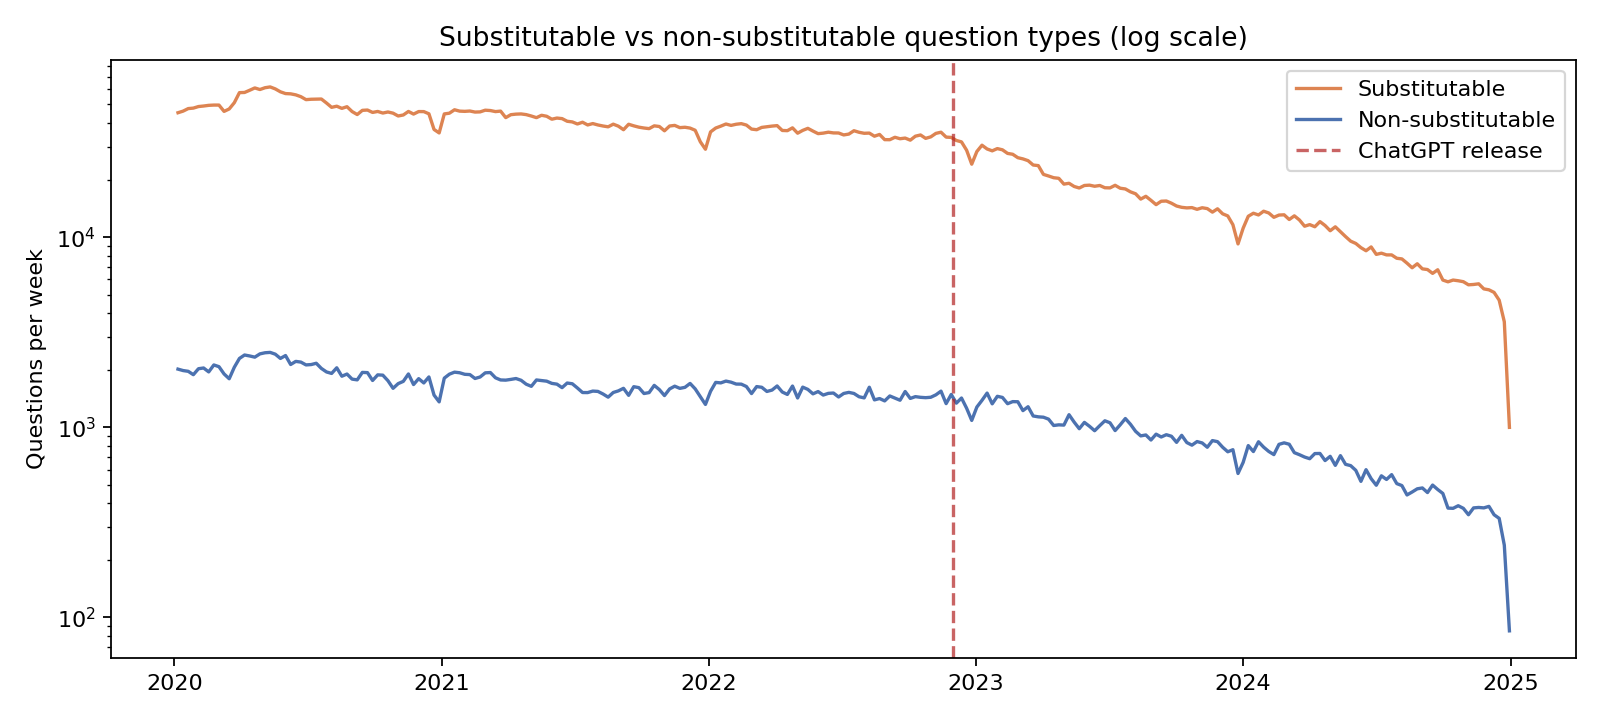
\includegraphics[width=0.82\textwidth]{figures/macro_substitutable_vs_not_log.png}
\caption{Weekly questions by substitutability, 2020--2024 (log
scale). Vertical line: ChatGPT release.}
\label{fig:macro_sub_vs_not}
\end{figure}

\subsection{Baseline DDD coefficient}\label{ssec:main_baseline}

The conservative inclusive baseline---retaining
advanced-architecture questions in the control and using the
full sample with the historical answerability index---is
$\hat\beta_{\text{DDD}}=-0.108$ (CR1 SE $0.046$, $p=0.021$).
Our preferred specification excludes the declared boundary
category advanced-architecture from the control
(\S\ref{ssec:data_ai_answerability}) and gives $-0.140$
($p=0.005$); restricting the substitutability label to the
high-agreement subsample gives $\approx-0.11$. The treatment
is measured two ways: the historical index and a co-primary
embedding-based answerability score that uses \emph{no} Stack
Overflow historical features ($-0.119$, $p<0.001$). The two
measures share none of their inputs, so we read the gradient
as answerability-driven rather than historical popularity,
without overselling their $r\approx0.4$--$0.5$ convergence as
more than moderate. The full robustness battery (alternative
proxies, sub-samples, leave-one-out, PPML, two-way
clustering, wild bootstrap, and a 32-cell specification curve
that is negative and significant in 100\% of cells) is in the
replication package.

\subsection{Support-post funnel}\label{ssec:results_funnel}

Existing displacement studies measure platform activity
(new questions). From a knowledge-production perspective the
relevant outcome is the production of posts that pass
observable support gates: answered, accepted by the asker,
not closed, and non-negative in net score---a
\emph{funnel-qualified post}. The term is deliberately
narrower than durable reuse, which the public data do not
observe; each gate is meaningful because it is operated by a
different actor (answerer, asker, moderator, crowd). We build
a five-transition funnel at the (tag, week, question-type)
cell from the $8{,}404{,}411$-question stream; only $38.0\%$
survive to the funnel-qualified stage. Re-fitting the
baseline DDD with each funnel stage as the outcome
(Table~\ref{tab:reusable_funnel}) gives a relative
coefficient that is stable across stages
($-0.108$ to $-0.121$, all $p<0.05$), so the implied
cumulative shortfall over the 109 post-ChatGPT weeks
contracts from $\sim$70{,}000 missing questions to
$\sim$28{,}000 missing funnel-qualified posts (about $40\%$
of the activity shortfall). The stability is partly
mechanical---the gates are nested---so the funnel is best
read as an operational accounting device from the volume
coefficient to observed support counts, not as evidence on
where in the value distribution the channel falls; that is
the value-weighted question we test next.

\begin{table}[ht]
\centering
\caption{Triple-difference (DDD) estimates across the observed support-post funnel. The dependent variable is $\log(1+Y_{twk})$ where $Y$ is the cell-level count. Coefficients on the triple interaction $\text{AI}_k \cdot \text{Post}_t \cdot \text{Sub}_k$ are reported, with tag-clustered standard errors in parentheses. The implied shortfall is computed as $\sum_{\text{post}}(Y \cdot e^{-\hat\beta \cdot \text{AI} \cdot \text{Sub}} - Y)$.}
\label{tab:reusable_funnel}
\small
\setlength{\tabcolsep}{4pt}
\begin{adjustbox}{max width=\textwidth}
\begin{tabular}{lrrrrrr}
\toprule
Funnel stage & $\hat\beta_{DDD}$ & SE & $p$ & 95\% CI & N obs & Implied shortfall \\
\midrule
Questions & -0.1082 & (0.0460) & 0.0206 & [-0.199, -0.017] & 164,351 & 70,364 \\
Answered & -0.1150 & (0.0463) & 0.0147 & [-0.207, -0.023] & 164,351 & 61,210 \\
Accepted answer & -0.1168 & (0.0476) & 0.0159 & [-0.211, -0.022] & 164,351 & 32,809 \\
Accepted, not closed & -0.1210 & (0.0480) & 0.0134 & [-0.216, -0.026] & 164,351 & 31,836 \\
Accepted, score $\geq 0$ & -0.1154 & (0.0484) & 0.0190 & [-0.211, -0.019] & 164,351 & 28,504 \\
Funnel-qualified post & -0.1183 & (0.0487) & 0.0169 & [-0.215, -0.022] & 164,351 & 28,001 \\
\bottomrule
\end{tabular}
\end{adjustbox}
\end{table}


\subsection{Value-weighted posts: the benign-pruning
test}\label{ssec:results_value_weighted}

The benign-pruning reading of the aggregate contraction
\citep{xue2026chatgpt} predicts that the channel concentrates
on the low-value end: LLMs absorb routine, low-score queries
that public Q\&A would not have retained in any case. We test
this at the within-tag value margin by re-fitting the DDD on
posts cut by crowd-validation score (in the raw stream, $51\%$
of funnel-qualified posts reach score $\geq1$ and only $4\%$
reach score $\geq5$).

\paragraph{A single pre-specified shape test (primary C1).}
To avoid resting the claim on a family of per-threshold tests,
we pre-specify one statistic (Table~\ref{tab:shape_test}):
stacking the six mutually exclusive net-score bins in one
model, we fit the triple difference plus its interaction with
the centred score level. The \emph{average} displacement
across the value distribution is $-0.167$ ($p<10^{-4}$)---a
single, clearly negative coefficient establishing that the
channel is not confined to score-zero posts---and the
\emph{slope} over score is $-0.094$ ($p=2\times10^{-4}$),
quantifying attenuation toward the elite tail. This is our
primary statement of C1.

\begin{table}[ht]
\centering
\caption{Pre-specified shape test of the value gradient. A single model stacks the six mutually exclusive net-score bins and fits the triple difference plus its interaction with the (centred) net-score level, clustered by tag. The \emph{average} coefficient tests whether the displacement is present across the value distribution (the focal C1 hypothesis); the \emph{slope} tests how it varies with score. This replaces multiple per-bin tests with one declared statistic.}
\label{tab:shape_test}
\small
\begin{tabular}{lrr}
\toprule
Quantity & Estimate & $p$ \\
\midrule
Average displacement across bins & -0.167 & 0.000 \\
Slope over net-score level & -0.094 & 0.000 \\
\bottomrule
\end{tabular}
\end{table}

\paragraph{Consistent corroboration.}
The mutually exclusive bins are flat across the low-to-mid
range ($-0.21$, $-0.20$, $-0.21$ at score $0,1,2$) and
attenuate above ($-0.164$, $-0.124$, $-0.091$ at $3,4,\geq5$);
bins $0$ through $4$ are each individually significant at
$p<0.005$ and survive a Bonferroni correction, so the
\emph{strict} benign-pruning hypothesis (displacement confined
to score-zero posts) is rejected by four separately
significant non-zero-score bins. The elite-tail bin
(score $\geq5$, $-0.091$, $p=0.116$) is underpowered
(MDE $0.16$) and we take its raw null at face value. A
conservative Romano--Wolf correction over the \emph{nested
cumulative} thresholds---which folds the underpowered elite
tail into every statistic---places that particular gradient at
the $10\%$ joint level; we report it in the replication
package as a stringent joint lens, not the headline. The
honest reading is therefore the \emph{shape}: displacement is
roughly proportional across the crowd-validated range and
fades only at the elite tail.

\subsection{Dynamics, pre-trends, and
placebos}\label{ssec:dynamics_event}

The quarterly event-study coefficient is negative and
significant in every post-treatment bin, growing
monotonically from $-0.063$ at $T{+}0$ to $-0.544$ at
$T{+}8$ (Q4 2024); pre-period coefficients are smaller (about
a third of the post mean) and converge toward zero as the
cutoff approaches (Figure~\ref{fig:event_study}).

\begin{figure}[!htbp]
\centering
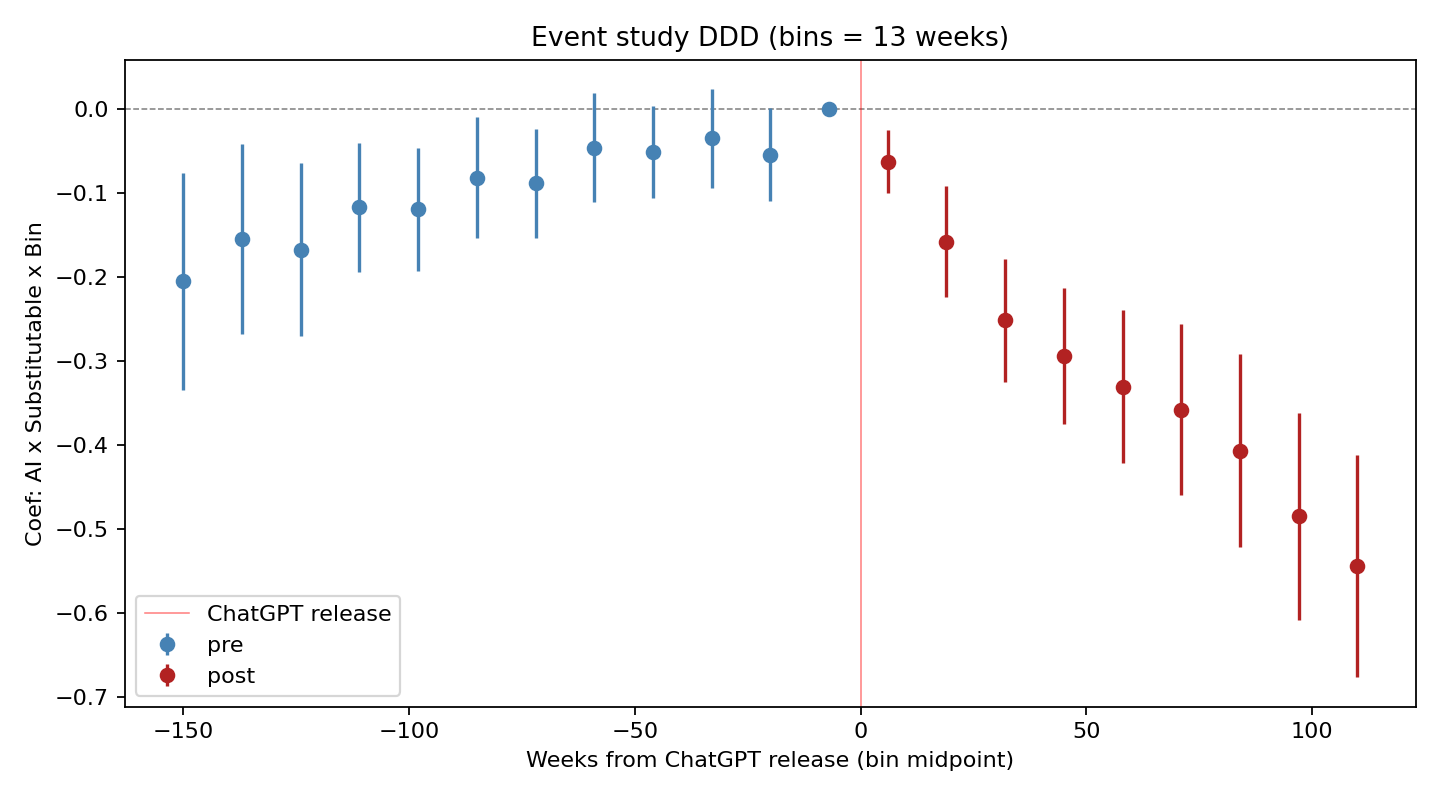
\includegraphics[width=0.82\textwidth]{figures/event_study_ddd_question_type_quarterly.png}
\caption{Quarterly event-study coefficients on
$\text{AI}\times\text{Sub}\times\text{bin}$. Reference: bin
$-1$ (immediately pre-treatment).}
\label{fig:event_study}
\end{figure}

Formal pre-trend tests reject exact parallel trends, so we do
not claim a standalone natural experiment; the estimates are
conditional post-ChatGPT associations whose credibility rests
on a conjunction of diagnostics. Under the official HonestDiD
$\Delta^{\text{RM}}$ implementation the breakdown is
$\bar M = 0.75$ (the robust 95\% CI first contains zero at
$\bar M = 0.75$; it remains $[-0.136,-0.010]$ at
$\bar M = 0.50$), which we read as a moderate signal. Five
conventional pre-period placebos return \emph{positive}
coefficients ($+0.059$ to $+0.067$, all $p<0.012$), and a
29-step rolling-placebo sweep (mean $+0.057$) contains no
cutoff as negative as the real one---a sign reversal hard to
reconcile with a smooth continuation of the pre-period path.
A June 2022 GitHub Copilot placebo is also positive
($+0.058$, $p=0.011$); in a joint model the ChatGPT
interaction is $-0.157$ ($p<0.001$) while Copilot stays
$+0.058$. Full event-study, placebo, and specification-curve
detail is in the replication package.

\subsection{Magnitude}\label{ssec:magnitude}\label{ssec:magnitude_benchmarks}

Applying the coefficient cell-by-cell to the post-period
panel implies $\sim$70{,}000 missing questions over the 109
post-ChatGPT weeks---$4.2\%$ of the $1{,}671{,}197$ observed
post-period questions in the top-100-tag panel. The implied
displaced high-value (score $\geq1$) flow is $\sim$15{,}200
posts ($0.9\%$ of all observed questions). Whether this small
flow matters is a stock--flow question: the public archive is
a durable stock, so a persistent reduction in the high-value
\emph{flow} ($\sim$7{,}300 posts/year at the window average)
accumulates to $\sim$36{,}000 over five years under a constant
flow. We present these as transparent projections under stated
assumptions, not forecasts, and they do not bear on welfare or
generalise beyond the panel. Benchmarked against a descriptive
linear extrapolation of the pre-trend ($\sim$1.42 million
questions), the DDD-estimated channel is about $5\%$---a
\emph{discipline} on causal interpretation: the aggregate
decline cannot all be attributed to LLM substitutability
without further identification.


\section{Robustness and validity}\label{sec:robustness}
\label{sec:robustness_body}

The headline finding survives the full battery (consolidated in
the replication package): the four alternative AI-answerability
measures (structural, $z$-score, PCA, quartile), the sub-sample
restrictions (top-50, top-75, leave-one-out of the top tags by
pre-volume), the continuous embedding substitutability score
($-0.039$, $p=0.004$), the alternative outcomes (unique users,
fractional tag counts), and the alternative inference (two-way
clustering, wild cluster bootstrap $p<0.005$, PPML $-0.098$,
$p=0.027$). The HonestDiD $\Delta^{\text{RM}}$ exercise
(\S\ref{ssec:id_honest_did}) breaks down at $\bar M=0.75$---a
moderate signal read together with the placebo sign-reversal and
the Copilot positive placebo ($+0.058$, $p=0.011$), which hold
independently of any smoothness restriction. The substitutability
classifier has only moderate multi-rater agreement (Fleiss
$\kappa=0.52$); we address this directly via the high-agreement
subsample (\S\ref{sec:validation}). Because exact parallel trends
are rejected, we emphasise the pre-slope-matched specification
(75 near-median tags, $-0.155$, $p=0.009$) as a central stress
test rather than an optional add-on.


\section{Mechanisms}\label{sec:mechanisms}
\label{sec:mechanisms_body}

\subsection{Decomposition by question type}\label{ssec:mech_by_type}\label{ssec:mech_qtype_anomaly}

Estimating the AI$\times$Post interaction separately for each
question type (tag and week fixed effects) orders the
coefficients as the substitutability theory predicts:
short-code ($-0.31$), how-to ($-0.28$), long-code ($-0.21$),
debugging-simple ($-0.14$), other-conceptual ($-0.08$,
marginal), advanced-architecture ($-0.16$, $p=0.003$), and
version-environment-specific (null, $-0.03$, $p=0.54$). The
version-environment-specific null---the genuinely clean
control---is the only category with no detected decline. That
the declared boundary category advanced-architecture shows a
sizeable effect confirms its a-priori boundary status
(\S\ref{ssec:data_ai_answerability}); because the binary
classifier codes it $\text{Sub}_k=0$, it contributes a negative
shift to the control group and mechanically attenuates the full
sample, which is why excluding it strengthens the funnel DDD
from $-0.108$ to $-0.140$ (full table in the replication
package). Replacing the binary indicator with the continuous
embedding score gives $-0.039$ ($p=0.004$), about a third the
binary magnitude as expected from shrinking the contrast; the
qualitative conclusion is unchanged.

\subsection{Composition versus within-cell
quality}\label{ssec:mech_complementarity}\label{ssec:mech_resolvability}

A complementarity reading holds that users keep posting when an
LLM answer is unsatisfactory, so the \emph{surviving} questions
should be more complex. Descriptively this holds: within tags,
post-period body length rises ($+303$ characters, $p<10^{-15}$)
and accepted-answer share falls ($-0.065$, $p<10^{-15}$). But
the Post$\times$AI-answerability interactions are null
($p$ between $0.32$ and $0.79$), so the compositional shift is
\emph{general across tags} rather than concentrated where
answerability is highest---it is descriptive selection, not a
causally estimated quality effect along the AI dimension.

Separating selection from a within-cell quality channel is the
contribution here. \citet{xue2026chatgpt} report higher average
question quality post-ChatGPT under a cross-platform design that
admits both channels. Re-fitting the DDD on six resolvability
and quality outcomes under fine-grained (tag$\times$question-type)
and week fixed effects---which absorb the composition shift---five
of six estimates are null (accepted share $-0.003$, $p=0.45$;
answered share $-0.001$, $p=0.85$; analogous nulls elsewhere);
the only significant coefficient is a small \emph{rise} in
closed share ($+0.005$, $p<0.001$). The descriptively documented
quality improvement is therefore consistent with selection into
the survivor population (the easier posts displaced into private
channels) rather than with within-cell upgrading. This is not a
contradiction of \citet{xue2026chatgpt}: the cross-platform ATT
(aggregate declines of $\sim$15--25\%;
\citealp{delriochanona2024large}) and the within-platform
$\sim$5\% slice estimated here are complementary objects, not
competing estimates of the same quantity (full mapping and
detail tables in the replication package).

\subsection{Where in the workflow does substitution
operate?}\label{ssec:mech_copilot}

The June 2022 GitHub Copilot placebo is positive ($+0.058$,
$p=0.011$): the Stack Overflow Q\&A margin responded to ChatGPT
but not to Copilot. Two non-exclusive readings are consistent
with the data and we cannot separate them: Copilot operated
inside the IDE at the code-writing moment rather than the
search-for-help moment that ends in a public query, and its 2022
user base was much smaller than ChatGPT's. The \emph{positive}
sign is the informative part (a shared secular trend cannot
produce it), but its magnitude rests on the smaller 2022
population, so the test has limited power; we read it as
supporting evidence on the decision-point reading, not a
stand-alone mechanism, and present any interface-location
interpretation as a post-hoc hypothesis the design does not
identify.


\section{Validation of question-type classification}\label{sec:validation}
\label{sec:validation_body}

The substitutable / non-substitutable binary classification is
the central measurement decision. The baseline classifier is
heuristic (title-keyword patterns plus body-length and
code-block features, mapped to seven categories then collapsed to
a binary label). We validate it against two independent
sentence-embedding classifiers on a stratified random sample of
10{,}000 questions: \texttt{all-MiniLM-L6-v2} and
\texttt{all-mpnet-base-v2} (different architectures and training
corpora, so their mutual agreement is a stronger signal than
either with the heuristic), each assigning questions to the
nearest category centroid in cosine space.

\subsection{Agreement and the high-agreement
subsample}\label{ssec:val_kappa}\label{ssec:val_high_agree}\label{ssec:val_protocol}\label{ssec:val_crosstab}\label{ssec:val_implications}

The two embedding classifiers agree with each other in the
substantial range (binary Cohen's $\kappa=0.67$; 7-way $0.68$),
above either's agreement with the heuristic ($\kappa=0.44$--$0.46$
binary), and the multi-rater Fleiss' $\kappa$ is $0.52$ for the
binary label and $0.40$ for the seven-way category---moderate
rather than strong. For $70.5\%$ of the sample all three
classifiers agree on the binary label, and within this
high-agreement subsample the DDD point estimate is statistically
indistinguishable from the full-sample baseline ($\approx-0.11$),
so the result is not driven by the heuristic's disagreement
cases. The heuristic is more conservative than the embedding
majority (labelling $28.6\%$ versus $22.4\%$ non-substitutable),
which under-counts non-substitutable cells and if anything
attenuates $\beta_{\text{DDD}}$. The substitutability concept
thus has reasonably stable semantic content across embeddings,
while the noisier seven-way split ($\kappa=0.40$) means the
question-type decomposition (\S\ref{ssec:mech_by_type}) should be
read as illustrative of the gradient---consistent with the
negative advanced-architecture coefficient---rather than as
precise category-by-category estimates. We retain the
embedding-validated heuristic as the funnel-building baseline and
use the continuous embedding score as a co-primary check; a
contemporary-LLM scorer would embed a specific model generation
into the measure and introduce circularity, which the zero-budget
design avoids. Full $\kappa$ tables and the cross-tabulation are
in the replication package.


\section{A value-calibrated early-warning system and its
implications}\label{sec:policy}
\label{sec:policy_body}

The empirical results have a direct operational use: they
specify a decision rule for monitoring whether the post-ChatGPT
contraction is reaching the crowd-validated margin in a given
tag or portfolio.

\subsection{A value-calibrated early-warning system}
\label{ssec:pol_monitor}

A platform manager allocating scarce intervention effort
(contributor incentives, attribution mechanisms, moderation
attention) needs two things: a \emph{detection} signal for which
tags are losing high-value reusable flow, and a way to
\emph{size} the high-value consequence of a detected decline. We
build a tool that does both, and we let the data choose the
detection signal rather than assume our value index is it.

The decision has two margins. At the \emph{extensive} margin
(which tags to act on), a value-disproportionality \emph{ratio}
(VtD) is a poor detector---on the full 100-tag panel it ranks
realised 2025 high-value erosion at AUC $0.57$, far below the
activity-decline metric a platform already tracks (AUC $0.98$,
out of sample). This high AUC is not interpreted as an
independent behavioural prediction---its detection target contains
activity-derived high-value erosion---but as evidence that the
operational activity signal is sufficient for triage; the value of
calibration is evaluated separately by the budgeted-regret
experiment below. The practical conclusion is that platforms need
no bespoke value instrumentation to \emph{detect} where erosion is
largest: the system detects on activity. At the \emph{intensive}
margin (how much effort per selected tag), the value calibration
earns its place: allocating an intervention budget by the
value-calibrated high-value-at-risk (activity scaled by the
tag's high-value share) nearly attains the perfect-foresight
optimum (calibrated regret under $1\%$), whereas allocating by \emph{raw}
activity leaves regret of $3$--$5\%$ of the protectable
high-value flow (Table~\ref{tab:vtd_voi}, full panel,
out-of-sample on realised 2025 loss). The calibration thus has
positive, measurable value of information, even though it does
not---and need not---improve detection.

The artefact is therefore a \emph{value-calibrated} early-warning
system, not a value-detector. Its detection layer is the
activity signal (AUC $0.98$); its contribution is the
\emph{calibration} layer that converts an activity alert into the
decision-relevant quantity a manager lacks: for a flagged tag $t$,
$\widehat{\text{HV}}_t = (\text{activity deficit}_t)\times(\text{tag
high-value share})$, the activity signal scaled by the
value-margin gradient of \S\ref{ssec:results_value_weighted}; a
loss-derived threshold sets the alert cutoff from costs rather
than a mechanical mean. The value-disproportionality index
survives in a strictly secondary role---it describes \emph{what
kind} of decline a tag has (it is cross-sectionally orthogonal to
the activity level, $\rho=0.08$; Figure~\ref{fig:vtd_monitor}),
and that classification persists from 2024 onto the new 2025 data
($\rho=0.90$, $p<0.001$), so a manager can use it to choose
intervention \emph{type} (high-value-contributor retention for
value-disproportionate tags versus generic re-engagement for
proportional ones). The system is provided as a reproducible
script run on quantities a platform already records; it is
\emph{not} a deployed interface, and we run no manager user study.
A production dashboard and usability evaluation are future work
(\S\ref{sec:limitations}).

\begin{table}[ht]
\centering
\caption{Intensive-margin value of calibration, \textbf{full 100-tag 2025 panel} (out of sample). A manager allocates an intervention budget $B$ (a fraction of total tag activity) to protect realised 2025 high-value flow, ranking by efficiency. \textbf{Oracle} is the perfect-foresight cost-constrained optimum; \textbf{Calibrated} ranks by end-2024 high-value-at-risk; \textbf{Naive} by raw activity loss; \textbf{Random} averages shuffles. Cells are the share of realised 2025 high-value loss captured; the regret of a rule is $(\text{Oracle}-\text{rule})/\text{Oracle}$.}
\label{tab:vtd_voi}
\small
\begin{tabular}{lrrrrrr}
\toprule
$B$ & Oracle & Calibrated & Naive & Random & Regret$_{\text{calib}}$ & Regret$_{\text{naive}}$ \\
\midrule
10\% & 0.19 & 0.19 & 0.19 & 0.08 & 0.01 & 0.04 \\
25\% & 0.38 & 0.38 & 0.36 & 0.23 & 0.00 & 0.05 \\
40\% & 0.55 & 0.55 & 0.52 & 0.38 & 0.00 & 0.04 \\
50\% & 0.65 & 0.64 & 0.63 & 0.48 & 0.00 & 0.03 \\
\bottomrule
\end{tabular}
\end{table}

\begin{figure}[!htbp]
\centering
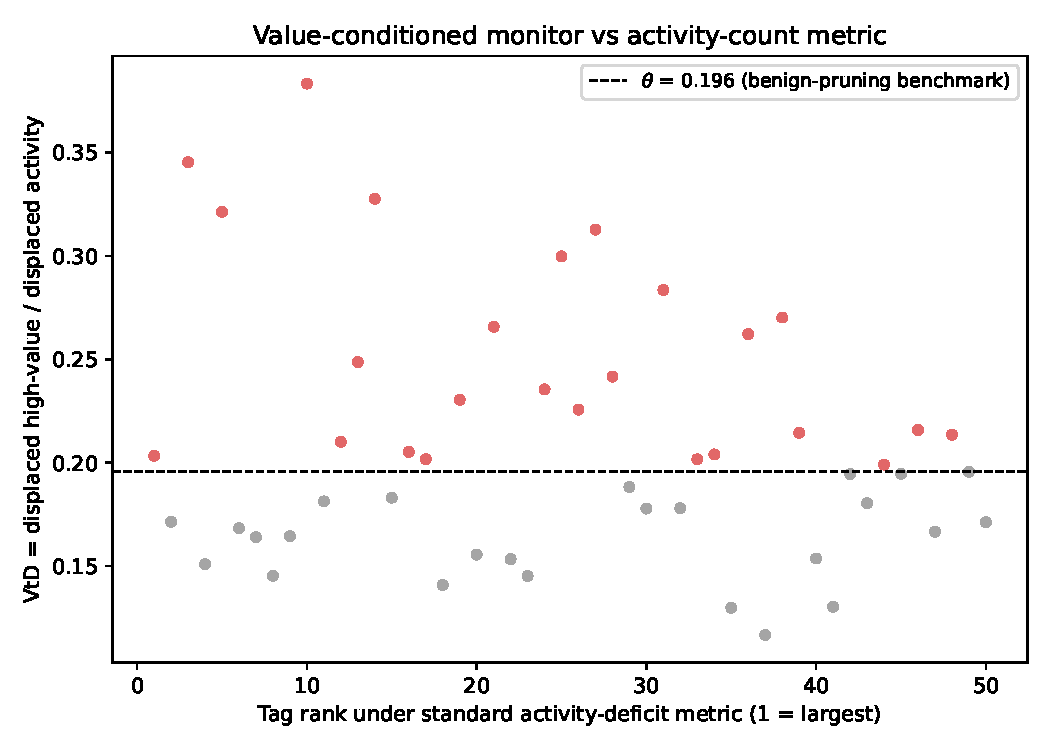
\includegraphics[width=0.78\textwidth]{figures/fig_vtd_monitor.pdf}
\caption{Value disproportionality versus the activity-count
metric. Each point is a tag, positioned by its activity-deficit
rank (horizontal) and VtD ratio (vertical); red points exceed the
benign-pruning benchmark $\theta=0.196$. The flat scatter
($\rho=0.08$) shows value disproportionality is close to
orthogonal to the \emph{size} of a tag's deficit. The activity
deficit remains the better predictor of erosion \emph{magnitude};
the monitor's contribution is the persistent disproportionality
dimension.}
\label{fig:vtd_monitor}
\end{figure}

\subsection{Implications for providers, managers, and
regulators}\label{ssec:pol_ai_providers}\label{ssec:pol_managers}\label{ssec:pol_regulators}\label{ssec:pol_welfare}

The asymmetry between activity and value is decision-relevant.
An AI provider or platform manager inferring training-corpus or
knowledge-production contraction from \emph{raw} post counts
overstates the funnel-qualified-post loss by a factor of roughly
$70{,}000/28{,}000\approx2.5$, because only about $40\%$ of raw
posts survive the support gates; and the value evidence
(\S\ref{ssec:results_value_weighted}) shows the displacement at
the crowd-validated tail is at least as strong relative to the
volume baseline. The dynamic concern that recursive training on
generated content degrades model quality
\citep{shumailov2024curse} gives providers a self-interested
reason to support attribution and contribution mechanisms (e.g.\
the May 2024 Stack Exchange--OpenAI agreement
\citep{stackexchange_openai_2024}). For regulators---e.g.\ the
training-data transparency provision of the EU AI Act
\citep{eu_ai_act_2024}---the sizing implication is that an
instrument framed on the LLM-substitutability margin should be
calibrated to the estimated channel ($\sim$5\% of the
trend-implied aggregate shortfall), not to the inferred
$65$--$71\%$ aggregate decline, which differs by an order of
magnitude. We do not estimate welfare and do not compare the
private productivity gains of LLM adoption against the public
shortfall: the two are in different units with different
horizons, and a static comparison would understate the dynamic
and distributional dimensions.

\subsection{What the magnitude does not
support}\label{ssec:pol_not_supported}

We do \emph{not} derive from the estimate: a welfare conclusion
(neither side of the trade-off is identified); an optimal-policy
recommendation (the social value of the marginal question is not
identified); an effect on innovation \emph{outcomes} (the DDD
estimates an innovation \emph{input}, not patents, products,
entry, or productivity); a generalisation beyond programming;
or a managerial intervention design (we do not identify the
elasticity of contribution to any specific instrument).


\section{Limitations}\label{sec:limitations}
\label{sec:limitations_body}

\paragraph{Generalisability.}\label{ssec:lim_generalize}
Stack Overflow is one Q\&A platform in one domain (programming).
The decision point we identify---the search-for-help moment that
historically ended in a public query and now ends in an LLM
conversation---is a portable object that generates testable
hypotheses for medical, legal \citep{choi2022chatgpt}, and
academic Q\&A, implementable with the same design and API; we do
not undertake them here because each domain needs its own
substitutability taxonomy. We also do not observe other public
channels (Reddit, Discord, forums), so the DDD estimates changes
\emph{on} Stack Overflow but cannot distinguish movement to
private LLMs from movement to other public channels.

\paragraph{Input margin, not innovation outcomes.}\label{ssec:lim_scope}
The DDD estimates an innovation \emph{input}
(\S\ref{ssec:theory_qa_as_input}), not patents, products, entry,
or productivity; the informative horizon for downstream
propagation is probably 5--10 years and our window is two.
Heterogeneity by user tenure---the margin \citet{xue2026chatgpt}
study---is not separately observed in the aggregated cell-level
panel; a follow-up using the Stack Exchange data dump
(zero-budget but storage-intensive) could close this gap.

\paragraph{Measurement of substitutability.}\label{ssec:lim_measurement}
The binary classification is validated but imperfect (Fleiss
$\kappa=0.52$; seven-way $\kappa=0.40$;
\S\ref{sec:validation}), and the negative coefficient on
advanced-architecture (\S\ref{ssec:mech_qtype_anomaly}) suggests
the boundary moves as capabilities improve. The pre-treatment
proxy is not a direct LLM-capability benchmark; we report the
embedding-answerability treatment as a co-primary check, but a
direct pass-rate measure (a local open-weight model over sampled
pre-period questions) would be more precise and is a natural next
step within the zero-budget rule.

\paragraph{Pre-trends.}\label{ssec:lim_pretrend}
Exact parallel trends are rejected; we treat the pre-period
convergence, placebo sign-reversal, Copilot placebo, and the
HonestDiD $\Delta^{\text{RM}}$ profile (robust CI first contains
zero at $\bar M=0.75$; \S\ref{ssec:id_honest_did}) as evidence
against a simple secular-trend explanation, not proof of parallel
trends, and describe the causal reading as moderate rather than
strong. A quadratic trend control (in the replication package)
absorbs more of the effect mechanically by mimicking the shock
shape; we report it as a limit case.

\paragraph{No welfare conclusion.}\label{ssec:lim_welfare}
We bound one public-cost channel from above. The private
productivity gains documented elsewhere are first-order and
plausibly an order of magnitude larger
(\S\ref{ssec:pol_welfare}), and the long-run model-degradation
implications \citep{shumailov2024curse} are unresolved.

\paragraph{Scope of the artefact.}\label{ssec:lim_artefact}
The early-warning system is a reproducible scoring-and-alerting
script (\S\ref{ssec:pol_monitor}); a production dashboard and a
usability evaluation with platform moderators would be required
to claim a deployed, human-evaluated system, and neither was
available for this study. (The 2025 panel extension earlier
flagged as future work is now complete for all 100 tags and used
in \S\ref{ssec:id_threats}.)


\section{Conclusion}\label{sec:conclusion}
\label{sec:conclusion_body}

Public Q\&A platforms codify routine problem-solving and
distribute spillovers across future learners. ChatGPT sharply
reduced the marginal cost of obtaining the same service
privately, and the recent literature
\citep{burtch2024chatgpt,delriochanona2024large,xue2026chatgpt}
documents the resulting aggregate contraction together with an
apparent improvement in surviving question quality---a
combination compatible with a benign reading under which only
the low-value end is pruned. We test that reading at the
within-tag value margin.

Using a triple difference on 8.4 million questions (100 top
tags, 261 weeks, seven question types), the central finding
rejects the \emph{strict} benign-pruning reading: a single
pre-specified shape test returns a negative average displacement
across the value distribution ($-0.167$, $p<10^{-4}$) that is
roughly constant across the low-to-mid crowd-validated range and
fades only at the rare elite tail, so the channel is not confined
to score-zero posts (the exclusive bins $0$ through $4$ are each
individually significant and Bonferroni-robust; a conservative
Romano--Wolf correction over the nested cumulative thresholds
places the gradient at the $10\%$ joint level). The volume
baseline is $-0.108$ ($p=0.021$), strengthening to $-0.140$
($p=0.005$) once the a-priori boundary category
advanced-architecture is excluded, and negative and significant
in all 32 cells of a specification curve. Because exact pre-trend
tests reject, we read the estimate as a conditional post-ChatGPT
association, not a natural experiment: its credibility rests on a
sign-reversing placebo distribution, monotone event-study growth,
a pre-trend-matched design ($-0.129$), and a HonestDiD breakdown
at $\bar M=0.75$. Re-estimating on the full 100-tag panel
extended through 2025 strengthens the effect to $-0.172$
($p=0.002$), deepening to $-0.68$ with no reversion---most
consistent with sustained diffusion rather than a transient
episode.

We turn the result into a \emph{value-calibrated early-warning
system}: out of sample, an activity-decline signal detects where
high-value erosion is largest (AUC $0.98$ versus $0.57$ for a
value-weighted detector) and the value-margin estimates
calibrate that alert into the high-value posts at risk, with a
persistent composition flag ($\rho=0.90$) classifying
intervention type. We do not document an effect on innovation
\emph{outcomes}, contributor entry, or productivity, and we
derive no welfare conclusion; the Q\&A margin is an innovation
\emph{input}, and the private productivity gains of LLM adoption
are not estimated. The conceptual implication is that generative
AI changes the \emph{value composition}, not only the quantity,
of the public knowledge inputs that fuel open innovation---the
dimension that innovation policy and management research should
follow. The entire pipeline is reproducible from public,
zero-budget data; the full robustness, mechanism, and validation
detail is in the replication package.


% ---------------------------------------------------------------
% Extended robustness, mechanism, and validation outputs live in
% the public replication package (a research-data and code
% archive), not as journal supplementary material.
% ---------------------------------------------------------------

\section*{Data and code availability}
All evidence necessary to evaluate the main claims is reported in
the article. A public replication package provides the code,
data-construction scripts, audit logs, derived tables, and
extended robustness outputs needed to reproduce the analysis; it
is a research-data and code archive, not journal supplementary
material. Raw Stack Overflow content is not redistributed;
derived statistics and scripts to regenerate the data from public
sources are provided where licensing permits. Replication
repository: \url{https://github.com/hlaverde/so-genai-value-margin}.

\bibliographystyle{plainnat}
\bibliography{references}

\end{document}
